%% This is file `tlsflyleaf.tex',
%% Copyright 2013 Tristan GREGOIRE
%
% This work may be distributed and/or modified under the
% conditions of the LaTeX Project Public License, either version 1.3
% of this license or (at your option) any later version.
% The latest version of this license is in
%   http://www.latex-project.org/lppl.txt
% and version 1.3 or later is part of all distributions of LaTeX
% version 2005/12/01 or later.
%
%
% This work has the LPPL maintenance status `maintained'.
% 
% The Current Maintainer of this work is T. GREGOIRE
%

\documentclass{scrartcl}

% ============================================================
% PACKAGE
\usepackage{fixltx2e}
\usepackage{etex}
\usepackage{lmodern}
\usepackage[T1]{fontenc}
\usepackage[utf8]{inputenc}
\usepackage{textcomp}
\usepackage{microtype}
\usepackage{hyperref}
\usepackage{listings}
\usepackage{color}
\usepackage{graphicx}
\usepackage[toc]{multitoc}
\usepackage{tocloft}
\usepackage{wasysym}

\hypersetup{linktocpage,
    colorlinks,
    citecolor=blue,
    filecolor=blue,
    linkcolor=blue,
    urlcolor=blue
}

\definecolor{dkgreen}{rgb}{0,0.6,0}
\definecolor{gray}{rgb}{0.5,0.5,0.5}
\definecolor{mauve}{rgb}{0.58,0,0.82}

\lstset{language=tex,
    tabsize=2,
    showstringspaces=false,
    basicstyle={\small\ttfamily},
    numbers=left,
    numberstyle=\tiny\color{gray},
    keywordstyle=\color{blue},
    commentstyle=\color{dkgreen},
    breaklines=true,
    breakatwhitespace=true,
    title=\lstname,
    escapeinside={\%*}{*)},
    frame=single
}


% ============================================================
% COMMAND
\newcommand*{\mail}[1]{\href{mailto:#1}{\texttt{#1}}}
\newcommand*{\www}[2]{\href{#2}{\texttt{#1}}}
\newcommand*{\pkg}[1]{\textsf{#1}}
\newcommand*{\cs}[1]{\texttt{\textbackslash#1}}
\makeatletter
\newcommand*{\cmd}[1]{\cs{\expandafter\@gobble\string#1}}
\makeatother
\newcommand*{\meta}[1]{\textlangle\textsl{#1}\textrangle}
\newcommand*{\marg}[1]{\texttt{\{}\meta{#1}\texttt{\}}}
\newcommand*{\opt}[1]{\texttt{#1}}
\newcommand*{\cmdarg}[1]{\{<\textit{#1}>\}}
\newcommand*{\file}[1]{\textit{\texttt{#1}}}

\addtokomafont{title}{\rmfamily}

% ============================================================
% TITLE
\title{The \pkg{pdgunivtls} package\thanks{This manual corresponds to \pkg{pdgunivtls.sty}~v1.1, dated~22 March 2013.}}
\author{Tristan GR\'EGOIRE\thanks{\mail{tlsflyleaf@onada.fr}}}
\date{22 March 2013}

% ============================================================
% DOCUMENT
\begin{document}
\maketitle

\begin{abstract}
	\noindent
	This package provide a simple comand \cmd{\makeflyleaf} that creates
	a flyleaf page for the PhD manuscript made at University of Toulouse.
\end{abstract}

\renewcommand{\cftsecleader}{\cftdotfill{\cftdotsep}}
\setlength\columnseprule{1pt}
\renewcommand\contentsname{\begin{center}\hrulefill \hspace*{1cm} Contents\hspace*{1cm} \hrulefill\end{center}}
\tableofcontents
~
\hrule


%%%%%%%%%%%%%%%%%%%%%%
\section{Introduction}
%%%%%%%%%%%%%%%%%%%%%%
This package provide a simple way to create and custom the official flyleaf of the University of Toulouse.
It is very usefull for PhD student who want write their PhD manuscript in \LaTeX{} and insert the official
flyleaf provide by the University in a private and not standard format.
Main use of this package is similar to the standard \cmd{\maketitle} with some stuff define
in the preambule of the \LaTeXe{} document and a single command (\cmd{\makeflyleaf}) used
in the body of the document to generate the flyleaf page.

%%%%%%%%%%%%%%%%%%%%%%
\section{Required package}
%%%%%%%%%%%%%%%%%%%%%%
\begin{enumerate}
    \item[\LaTeX{}] a recent \LaTeX{} installation $\ge$ 2011.
	\item[\pkg{shadowtext}] package: \pkg{shadowtext.sty}~v0.3, dated~2012/05/07 \\
	    \www{http://www.ctan.org/tex-archive/macros/latex/contrib/shadowtext}{http://www.ctan.org/tex-archive/macros/latex/contrib/shadowtext}
\end{enumerate}

%%%%%%%%%%%%%%%%%%%%%%
\section{Preamble}
%%%%%%%%%%%%%%%%%%%%%%
In the preamnble, you need to define all the contains of the flyleaf page information 
using very simple commands.
But before that you need to load the package using the simple commande line : \cmd{\usepackage[\textit{<option>}]{tlsflyleaf}}.
Option are very important and allow you to define the establishment name and the doctoral school to be print on the flyleaf (for more details on package option, see section~\ref{sec:opt}).
\begin{description}
    \renewcommand{\makelabel}[1]{#1}
	\item[\cmd{\title}\cmdarg{title}] French version of the Title of the PhD.
	\item[\cmd{\defencedate}\cmdarg{date}] defence date.
	\item[\cmd{\lab}\cmdarg{laboratory}] name of the laboratory.
	\item[\cmd{\author}\cmdarg{name}] name of the author.
  \item[\cmd{\nboss}\cmdarg{integer}] define the total number of `boss' to be printed (hereafter labeled as `\textit{\textbackslash npeople}'). Need to be in [1,2,3,\ldots].
    \item[\cmd{\nreferee}\cmdarg{integer}] define the total number of `referee' to be printed (hereafter labeled as `\textit{\textbackslash npeople}'). Need to be in [1,2,3,\ldots].
    \item[\cmd{\njudge}\cmdarg{integer}] define the total number of `judge' to be printed (hereafter labeled as `\textit{\textbackslash npeople}'). Need to be in [0,1,2,\ldots].
	\item[\cmd{\makesomeone}\cmdarg{category}\cmdarg{number}\cmdarg{name}\cmdarg{status>}\cmdarg{other}] Command that create "someone".
		Used to set a \textit{boss}, \textit{judge} or a \textit{referee}.
        \begin{description}
            \renewcommand{\makelabel}[1]{\textit{#1}}
            \item[<category>] should be select in [`boss', `referee', `judge']
            \item[<number>] is the rank for printing the person. 
                Only number $\le$ \textit{\textbackslash npeople} will be printed
            \item[<name>] First name and las name of the people
            \item[<status>] choose in "charg\'e de recherche", "professeur d'universit\'e" \ldots
            \item[<other>] What ever string you want to add (laboratory, jury member place\ldots).
        \end{description}

		This command need to be used with the \cmd{\nboss}, \cmd{\njudge} and \cmd{\nreferee}.
		Each \textit{\textbackslash npeople} command define the total number of people in each status to be printed.
  \item[\cmd{\cotutelle}\cmdarg{establishment}] define the international 'cotutelle' establishment name.
      \textbf{Don't use this command if you are not in 'cotutelle'.}
\end{description}
See sections \ref{sec:ex} for a simple but powerfull example.

%%%%%%%%%%%%%%%%%%%%%%
\section{Inside the document}
%%%%%%%%%%%%%%%%%%%%%%
Like for the standard command \cmd{\maketitle}, you only need to call the \cmd{\makeflyleaf} command to create the flyleaf page.

%%%%%%%%%%%%%%%%%%%%%%
\section{Package options\label{sec:opt}}
%%%%%%%%%%%%%%%%%%%%%%
\begin{enumerate}
	\item[\opt{emptysheetbefore}] Create two empty pages (that mean one sheet) before the flyleaf (see \opt{emptypageafter}).
	\item[\opt{emptypageafter}] Insert one empty page after the flyleaf. \\
		\opt{emptysheetbefore} and \opt{emptypageafter} are very usefull for example in the case of writing a book
		with odd and even pages. That allow an empty sheet before the flyleaf.
		Default behavior is to not insert those empty pages.
  \item[\opt{Ets=\textit{<value>}}] Define the establishment name in the flyleaf. No option given print a red message on the flyleaf. Value allowed for this option are provided in a full list in section~\ref{ssec:Ets}.
  \item[\opt{ED=\textit{<value>}}] Define the doctoral school and speciality. No option given print a red message on the flyleaf. A full list of value allowed for \opt{ED} is provided in section~\ref{ssec:ED}.
  \item[\opt{ED2=\textit{<value>}}] Allow the definition of a 'double mention' (second speciality). This option is optional: no option nothing done. The full list of value allowed is the same as for \opt{ED} (see section~\ref{ssec:ED}.
\end{enumerate}

%%%%%%%%%%%%%%%%%%%%%%
\section{Example\label{sec:ex}}
%%%%%%%%%%%%%%%%%%%%%%
\write18{pdflatex example.tex}
\lstinputlisting[firstline=18]{example.tex}
\begin{figure}[h!]
    \centering
    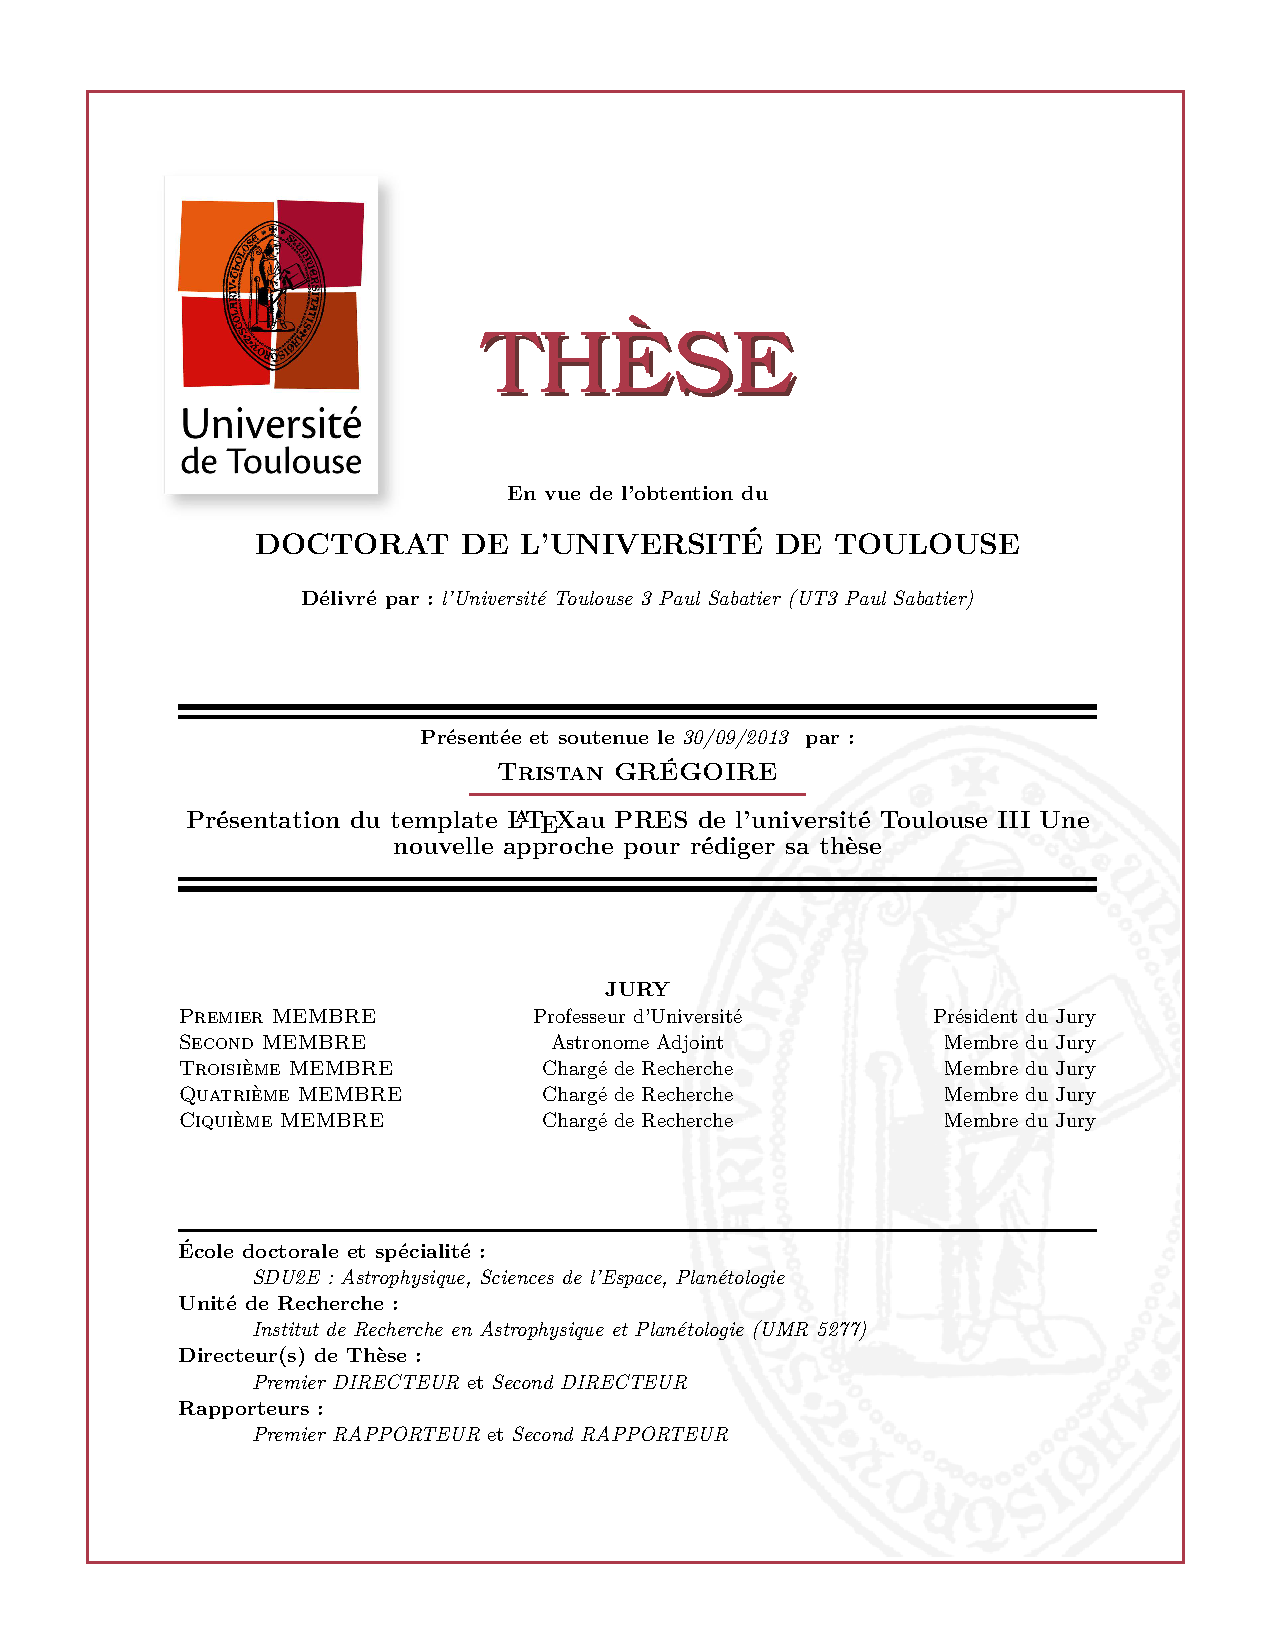
\includegraphics[width=\textwidth]{example.pdf}
    \caption{\label{fig:ex}
        Rendering for \LaTeX{} code of \file{example.tex} (shown in section~\ref{sec:ex}).
    }
\end{figure}
Rendering for this code is shown in Figure~\ref{fig:ex}.

%%%%%%%%%%%%%%%%%%%%%%
\section*{Appendix}
\addcontentsline{toc}{section}{Appendix}
%%%%%%%%%%%%%%%%%%%%%%
\subsection{Ets-list\label{ssec:Ets}}
Here you have the full list of establishment allowed by the package option \texttt{Ets} on the form:
\texttt{OptionValue -> Establishment}
\lstinputlisting[firstline=5]{ETS-list.txt}
\subsection{ED-list\label{ssec:ED}}
Here you have the full list of doctoral school and speciality allowed by the package option \texttt{ED} on the form :
\texttt{OptionValue -> Doctoral school : Speciality}.
\lstinputlisting[firstline=5]{ED-list.txt}


%%%%%%%%%%%%%%%%%%%%%%
\section*{Thanks}
\addcontentsline{toc}{section}{Thanks}
%%%%%%%%%%%%%%%%%%%%%%
Special thanks to Bastien and Simon for their ideas, comments and help.

\noindent This package has been developed by \textbf{Tristan GR\'EGOIRE}.
If you have any question, please fell free to contact me at \mail{tlsflyleaf@onada.fr}.

\medskip
\noindent\smiley \hfill Enjoy your PhD $\ddot\smile$. \hfill \smiley

\bigskip
\hfill \copyright{} Tristan GR\'EGOIRE, 2013

\end{document}
